% Created by tikzDevice version 0.10.1 on 2020-02-15 16:01:12
% !TEX encoding = UTF-8 Unicode
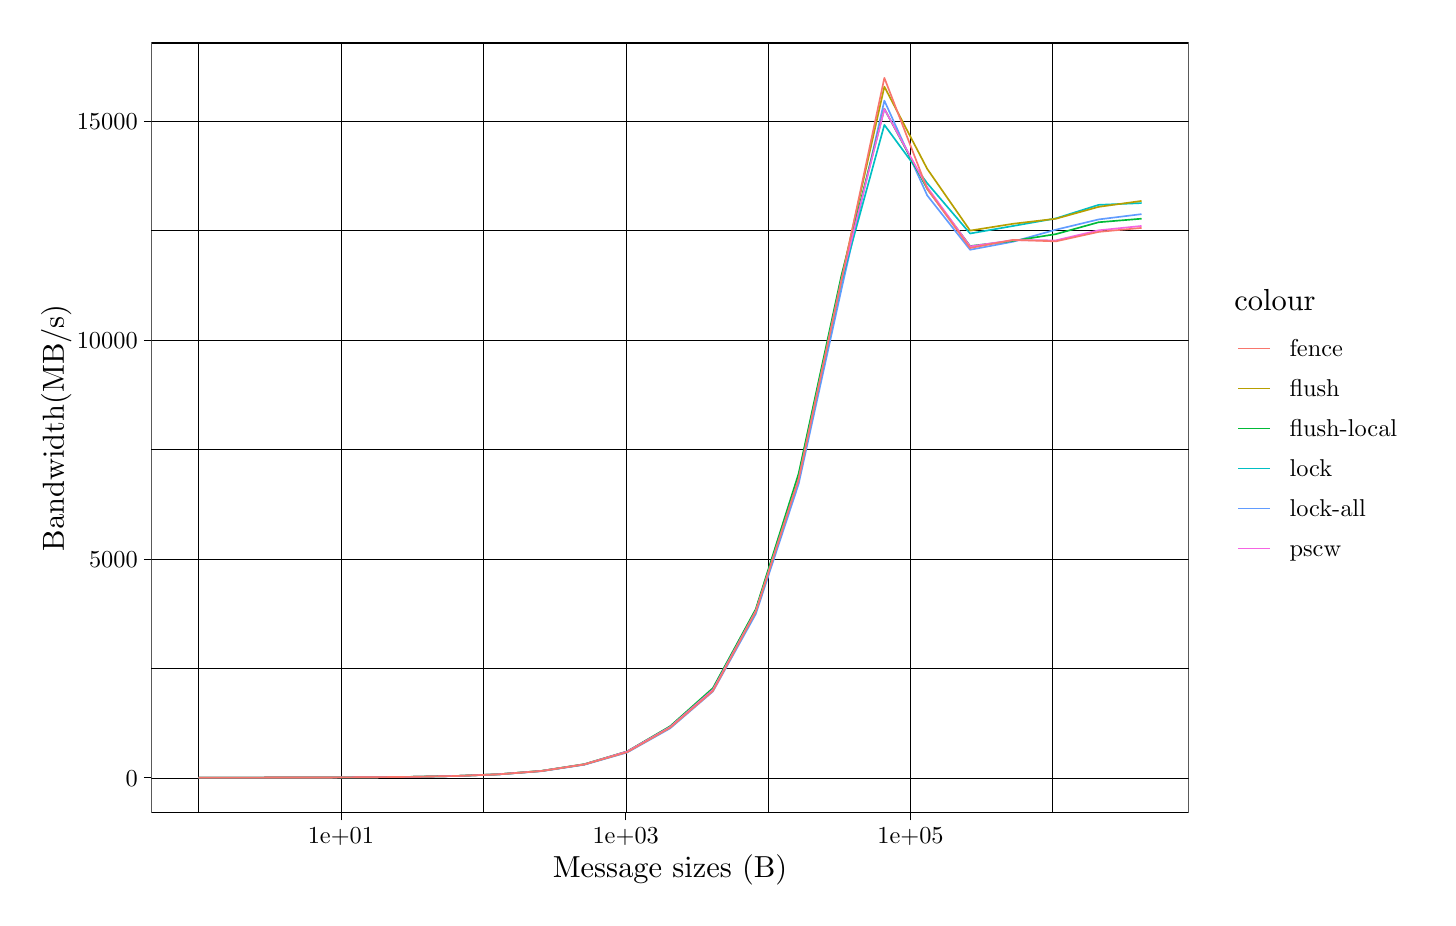
\begin{tikzpicture}[x=1pt,y=1pt]
\definecolor{fillColor}{RGB}{255,255,255}
\path[use as bounding box,fill=fillColor,fill opacity=0.00] (0,0) rectangle (505.89,314.37);
\begin{scope}
\path[clip] (  0.00,  0.00) rectangle (505.89,314.37);
\definecolor{drawColor}{RGB}{255,255,255}
\definecolor{fillColor}{RGB}{255,255,255}

\path[draw=drawColor,line width= 0.6pt,line join=round,line cap=round,fill=fillColor] (  0.00,  0.00) rectangle (505.89,314.37);
\end{scope}
\begin{scope}
\path[clip] ( 44.71, 30.72) rectangle (419.53,308.87);
\definecolor{fillColor}{RGB}{255,255,255}

\path[fill=fillColor] ( 44.71, 30.72) rectangle (419.53,308.87);
\definecolor{drawColor}{RGB}{0,0,0}

\path[draw=drawColor,line width= 0.0pt,line join=round] ( 44.71, 82.88) --
	(419.53, 82.88);

\path[draw=drawColor,line width= 0.0pt,line join=round] ( 44.71,161.91) --
	(419.53,161.91);

\path[draw=drawColor,line width= 0.0pt,line join=round] ( 44.71,240.94) --
	(419.53,240.94);

\path[draw=drawColor,line width= 0.0pt,line join=round] ( 61.75, 30.72) --
	( 61.75,308.87);

\path[draw=drawColor,line width= 0.0pt,line join=round] (164.65, 30.72) --
	(164.65,308.87);

\path[draw=drawColor,line width= 0.0pt,line join=round] (267.55, 30.72) --
	(267.55,308.87);

\path[draw=drawColor,line width= 0.0pt,line join=round] (370.46, 30.72) --
	(370.46,308.87);

\path[draw=drawColor,line width= 0.1pt,line join=round] ( 44.71, 43.36) --
	(419.53, 43.36);

\path[draw=drawColor,line width= 0.1pt,line join=round] ( 44.71,122.39) --
	(419.53,122.39);

\path[draw=drawColor,line width= 0.1pt,line join=round] ( 44.71,201.42) --
	(419.53,201.42);

\path[draw=drawColor,line width= 0.1pt,line join=round] ( 44.71,280.46) --
	(419.53,280.46);

\path[draw=drawColor,line width= 0.1pt,line join=round] (113.20, 30.72) --
	(113.20,308.87);

\path[draw=drawColor,line width= 0.1pt,line join=round] (216.10, 30.72) --
	(216.10,308.87);

\path[draw=drawColor,line width= 0.1pt,line join=round] (319.01, 30.72) --
	(319.01,308.87);
\definecolor{drawColor}{RGB}{97,156,255}

\path[draw=drawColor,line width= 0.6pt,line join=round] ( 61.75, 43.37) --
	( 77.24, 43.38) --
	( 92.73, 43.40) --
	(108.22, 43.43) --
	(123.70, 43.51) --
	(139.19, 43.66) --
	(154.68, 43.95) --
	(170.17, 44.54) --
	(185.66, 45.71) --
	(201.15, 48.04) --
	(216.63, 52.47) --
	(232.12, 61.17) --
	(247.61, 74.52) --
	(263.10,102.50) --
	(278.59,149.54) --
	(294.08,219.96) --
	(309.56,287.99) --
	(325.05,253.75) --
	(340.54,234.12) --
	(356.03,237.02) --
	(371.52,241.36) --
	(387.00,245.08) --
	(402.49,246.99);
\definecolor{drawColor}{RGB}{0,191,196}

\path[draw=drawColor,line width= 0.6pt,line join=round] ( 61.75, 43.37) --
	( 77.24, 43.38) --
	( 92.73, 43.40) --
	(108.22, 43.44) --
	(123.70, 43.51) --
	(139.19, 43.66) --
	(154.68, 43.96) --
	(170.17, 44.56) --
	(185.66, 45.76) --
	(201.15, 48.13) --
	(216.63, 52.67) --
	(232.12, 61.49) --
	(247.61, 75.02) --
	(263.10,103.29) --
	(278.59,151.19) --
	(294.08,222.60) --
	(309.56,279.24) --
	(325.05,258.16) --
	(340.54,239.99) --
	(356.03,242.70) --
	(371.52,245.44) --
	(387.00,250.34) --
	(402.49,250.99);
\definecolor{drawColor}{RGB}{183,159,0}

\path[draw=drawColor,line width= 0.6pt,line join=round] ( 61.75, 43.37) --
	( 77.24, 43.38) --
	( 92.73, 43.40) --
	(108.22, 43.44) --
	(123.70, 43.51) --
	(139.19, 43.66) --
	(154.68, 43.97) --
	(170.17, 44.58) --
	(185.66, 45.79) --
	(201.15, 48.19) --
	(216.63, 52.82) --
	(232.12, 61.73) --
	(247.61, 75.37) --
	(263.10,103.93) --
	(278.59,152.37) --
	(294.08,224.02) --
	(309.56,293.05) --
	(325.05,263.34) --
	(340.54,241.04) --
	(356.03,243.50) --
	(371.52,245.32) --
	(387.00,249.62) --
	(402.49,251.76);
\definecolor{drawColor}{RGB}{0,186,56}

\path[draw=drawColor,line width= 0.6pt,line join=round] ( 61.75, 43.37) --
	( 77.24, 43.38) --
	( 92.73, 43.40) --
	(108.22, 43.44) --
	(123.70, 43.51) --
	(139.19, 43.67) --
	(154.68, 43.98) --
	(170.17, 44.59) --
	(185.66, 45.82) --
	(201.15, 48.23) --
	(216.63, 52.84) --
	(232.12, 61.92) --
	(247.61, 75.72) --
	(263.10,104.26) --
	(278.59,153.25) --
	(294.08,224.93) --
	(309.56,285.05) --
	(325.05,256.13) --
	(340.54,235.46) --
	(356.03,237.31) --
	(371.52,239.76) --
	(387.00,244.06) --
	(402.49,245.34);
\definecolor{drawColor}{RGB}{245,100,227}

\path[draw=drawColor,line width= 0.6pt,line join=round] ( 61.75, 43.37) --
	( 77.24, 43.38) --
	( 92.73, 43.40) --
	(108.22, 43.44) --
	(123.70, 43.51) --
	(139.19, 43.66) --
	(154.68, 43.97) --
	(170.17, 44.58) --
	(185.66, 45.79) --
	(201.15, 48.18) --
	(216.63, 52.81) --
	(232.12, 61.65) --
	(247.61, 75.11) --
	(263.10,103.58) --
	(278.59,151.21) --
	(294.08,223.32) --
	(309.56,284.99) --
	(325.05,256.71) --
	(340.54,235.32) --
	(356.03,237.58) --
	(371.52,237.51) --
	(387.00,241.14) --
	(402.49,242.72);
\definecolor{drawColor}{RGB}{248,118,109}

\path[draw=drawColor,line width= 0.6pt,line join=round] ( 61.75, 43.37) --
	( 77.24, 43.38) --
	( 92.73, 43.40) --
	(108.22, 43.43) --
	(123.70, 43.51) --
	(139.19, 43.66) --
	(154.68, 43.96) --
	(170.17, 44.56) --
	(185.66, 45.76) --
	(201.15, 48.14) --
	(216.63, 52.58) --
	(232.12, 61.40) --
	(247.61, 74.68) --
	(263.10,103.33) --
	(278.59,151.27) --
	(294.08,223.22) --
	(309.56,296.23) --
	(325.05,256.10) --
	(340.54,234.73) --
	(356.03,237.68) --
	(371.52,237.15) --
	(387.00,240.58) --
	(402.49,242.01);
\definecolor{drawColor}{RGB}{0,0,0}

\path[draw=drawColor,line width= 0.6pt,line join=round,line cap=round] ( 44.71, 30.72) rectangle (419.53,308.87);
\end{scope}
\begin{scope}
\path[clip] (  0.00,  0.00) rectangle (505.89,314.37);
\definecolor{drawColor}{RGB}{0,0,0}

\node[text=drawColor,anchor=base east,inner sep=0pt, outer sep=0pt, scale=  0.88] at ( 39.76, 40.33) {0};

\node[text=drawColor,anchor=base east,inner sep=0pt, outer sep=0pt, scale=  0.88] at ( 39.76,119.36) {5000};

\node[text=drawColor,anchor=base east,inner sep=0pt, outer sep=0pt, scale=  0.88] at ( 39.76,198.39) {10000};

\node[text=drawColor,anchor=base east,inner sep=0pt, outer sep=0pt, scale=  0.88] at ( 39.76,277.43) {15000};
\end{scope}
\begin{scope}
\path[clip] (  0.00,  0.00) rectangle (505.89,314.37);
\definecolor{drawColor}{RGB}{0,0,0}

\path[draw=drawColor,line width= 0.3pt,line join=round] ( 41.96, 43.36) --
	( 44.71, 43.36);

\path[draw=drawColor,line width= 0.3pt,line join=round] ( 41.96,122.39) --
	( 44.71,122.39);

\path[draw=drawColor,line width= 0.3pt,line join=round] ( 41.96,201.42) --
	( 44.71,201.42);

\path[draw=drawColor,line width= 0.3pt,line join=round] ( 41.96,280.46) --
	( 44.71,280.46);
\end{scope}
\begin{scope}
\path[clip] (  0.00,  0.00) rectangle (505.89,314.37);
\definecolor{drawColor}{RGB}{0,0,0}

\path[draw=drawColor,line width= 0.3pt,line join=round] (113.20, 27.97) --
	(113.20, 30.72);

\path[draw=drawColor,line width= 0.3pt,line join=round] (216.10, 27.97) --
	(216.10, 30.72);

\path[draw=drawColor,line width= 0.3pt,line join=round] (319.01, 27.97) --
	(319.01, 30.72);
\end{scope}
\begin{scope}
\path[clip] (  0.00,  0.00) rectangle (505.89,314.37);
\definecolor{drawColor}{RGB}{0,0,0}

\node[text=drawColor,anchor=base,inner sep=0pt, outer sep=0pt, scale=  0.88] at (113.20, 19.71) {1e+01};

\node[text=drawColor,anchor=base,inner sep=0pt, outer sep=0pt, scale=  0.88] at (216.10, 19.71) {1e+03};

\node[text=drawColor,anchor=base,inner sep=0pt, outer sep=0pt, scale=  0.88] at (319.01, 19.71) {1e+05};
\end{scope}
\begin{scope}
\path[clip] (  0.00,  0.00) rectangle (505.89,314.37);
\definecolor{drawColor}{RGB}{0,0,0}

\node[text=drawColor,anchor=base,inner sep=0pt, outer sep=0pt, scale=  1.10] at (232.12,  7.44) {Message sizes (B)};
\end{scope}
\begin{scope}
\path[clip] (  0.00,  0.00) rectangle (505.89,314.37);
\definecolor{drawColor}{RGB}{0,0,0}

\node[text=drawColor,rotate= 90.00,anchor=base,inner sep=0pt, outer sep=0pt, scale=  1.10] at ( 13.08,169.80) {Bandwidth(MB/s)};
\end{scope}
\begin{scope}
\path[clip] (  0.00,  0.00) rectangle (505.89,314.37);
\definecolor{fillColor}{RGB}{255,255,255}

\path[fill=fillColor] (430.53,113.43) rectangle (500.39,226.17);
\end{scope}
\begin{scope}
\path[clip] (  0.00,  0.00) rectangle (505.89,314.37);
\definecolor{drawColor}{RGB}{0,0,0}

\node[text=drawColor,anchor=base west,inner sep=0pt, outer sep=0pt, scale=  1.10] at (436.03,212.12) {colour};
\end{scope}
\begin{scope}
\path[clip] (  0.00,  0.00) rectangle (505.89,314.37);
\definecolor{fillColor}{RGB}{255,255,255}

\path[fill=fillColor] (436.03,191.20) rectangle (450.48,205.65);
\end{scope}
\begin{scope}
\path[clip] (  0.00,  0.00) rectangle (505.89,314.37);
\definecolor{drawColor}{RGB}{248,118,109}

\path[draw=drawColor,line width= 0.6pt,line join=round] (437.48,198.42) -- (449.04,198.42);
\end{scope}
\begin{scope}
\path[clip] (  0.00,  0.00) rectangle (505.89,314.37);
\definecolor{drawColor}{RGB}{248,118,109}

\path[draw=drawColor,line width= 0.6pt,line join=round] (437.48,198.42) -- (449.04,198.42);
\end{scope}
\begin{scope}
\path[clip] (  0.00,  0.00) rectangle (505.89,314.37);
\definecolor{drawColor}{RGB}{248,118,109}

\path[draw=drawColor,line width= 0.6pt,line join=round] (437.48,198.42) -- (449.04,198.42);
\end{scope}
\begin{scope}
\path[clip] (  0.00,  0.00) rectangle (505.89,314.37);
\definecolor{drawColor}{RGB}{248,118,109}

\path[draw=drawColor,line width= 0.6pt,line join=round] (437.48,198.42) -- (449.04,198.42);
\end{scope}
\begin{scope}
\path[clip] (  0.00,  0.00) rectangle (505.89,314.37);
\definecolor{drawColor}{RGB}{248,118,109}

\path[draw=drawColor,line width= 0.6pt,line join=round] (437.48,198.42) -- (449.04,198.42);
\end{scope}
\begin{scope}
\path[clip] (  0.00,  0.00) rectangle (505.89,314.37);
\definecolor{drawColor}{RGB}{248,118,109}

\path[draw=drawColor,line width= 0.6pt,line join=round] (437.48,198.42) -- (449.04,198.42);
\end{scope}
\begin{scope}
\path[clip] (  0.00,  0.00) rectangle (505.89,314.37);
\definecolor{fillColor}{RGB}{255,255,255}

\path[fill=fillColor] (436.03,176.74) rectangle (450.48,191.20);
\end{scope}
\begin{scope}
\path[clip] (  0.00,  0.00) rectangle (505.89,314.37);
\definecolor{drawColor}{RGB}{183,159,0}

\path[draw=drawColor,line width= 0.6pt,line join=round] (437.48,183.97) -- (449.04,183.97);
\end{scope}
\begin{scope}
\path[clip] (  0.00,  0.00) rectangle (505.89,314.37);
\definecolor{drawColor}{RGB}{183,159,0}

\path[draw=drawColor,line width= 0.6pt,line join=round] (437.48,183.97) -- (449.04,183.97);
\end{scope}
\begin{scope}
\path[clip] (  0.00,  0.00) rectangle (505.89,314.37);
\definecolor{drawColor}{RGB}{183,159,0}

\path[draw=drawColor,line width= 0.6pt,line join=round] (437.48,183.97) -- (449.04,183.97);
\end{scope}
\begin{scope}
\path[clip] (  0.00,  0.00) rectangle (505.89,314.37);
\definecolor{drawColor}{RGB}{183,159,0}

\path[draw=drawColor,line width= 0.6pt,line join=round] (437.48,183.97) -- (449.04,183.97);
\end{scope}
\begin{scope}
\path[clip] (  0.00,  0.00) rectangle (505.89,314.37);
\definecolor{drawColor}{RGB}{183,159,0}

\path[draw=drawColor,line width= 0.6pt,line join=round] (437.48,183.97) -- (449.04,183.97);
\end{scope}
\begin{scope}
\path[clip] (  0.00,  0.00) rectangle (505.89,314.37);
\definecolor{drawColor}{RGB}{183,159,0}

\path[draw=drawColor,line width= 0.6pt,line join=round] (437.48,183.97) -- (449.04,183.97);
\end{scope}
\begin{scope}
\path[clip] (  0.00,  0.00) rectangle (505.89,314.37);
\definecolor{fillColor}{RGB}{255,255,255}

\path[fill=fillColor] (436.03,162.29) rectangle (450.48,176.74);
\end{scope}
\begin{scope}
\path[clip] (  0.00,  0.00) rectangle (505.89,314.37);
\definecolor{drawColor}{RGB}{0,186,56}

\path[draw=drawColor,line width= 0.6pt,line join=round] (437.48,169.52) -- (449.04,169.52);
\end{scope}
\begin{scope}
\path[clip] (  0.00,  0.00) rectangle (505.89,314.37);
\definecolor{drawColor}{RGB}{0,186,56}

\path[draw=drawColor,line width= 0.6pt,line join=round] (437.48,169.52) -- (449.04,169.52);
\end{scope}
\begin{scope}
\path[clip] (  0.00,  0.00) rectangle (505.89,314.37);
\definecolor{drawColor}{RGB}{0,186,56}

\path[draw=drawColor,line width= 0.6pt,line join=round] (437.48,169.52) -- (449.04,169.52);
\end{scope}
\begin{scope}
\path[clip] (  0.00,  0.00) rectangle (505.89,314.37);
\definecolor{drawColor}{RGB}{0,186,56}

\path[draw=drawColor,line width= 0.6pt,line join=round] (437.48,169.52) -- (449.04,169.52);
\end{scope}
\begin{scope}
\path[clip] (  0.00,  0.00) rectangle (505.89,314.37);
\definecolor{drawColor}{RGB}{0,186,56}

\path[draw=drawColor,line width= 0.6pt,line join=round] (437.48,169.52) -- (449.04,169.52);
\end{scope}
\begin{scope}
\path[clip] (  0.00,  0.00) rectangle (505.89,314.37);
\definecolor{drawColor}{RGB}{0,186,56}

\path[draw=drawColor,line width= 0.6pt,line join=round] (437.48,169.52) -- (449.04,169.52);
\end{scope}
\begin{scope}
\path[clip] (  0.00,  0.00) rectangle (505.89,314.37);
\definecolor{fillColor}{RGB}{255,255,255}

\path[fill=fillColor] (436.03,147.84) rectangle (450.48,162.29);
\end{scope}
\begin{scope}
\path[clip] (  0.00,  0.00) rectangle (505.89,314.37);
\definecolor{drawColor}{RGB}{0,191,196}

\path[draw=drawColor,line width= 0.6pt,line join=round] (437.48,155.06) -- (449.04,155.06);
\end{scope}
\begin{scope}
\path[clip] (  0.00,  0.00) rectangle (505.89,314.37);
\definecolor{drawColor}{RGB}{0,191,196}

\path[draw=drawColor,line width= 0.6pt,line join=round] (437.48,155.06) -- (449.04,155.06);
\end{scope}
\begin{scope}
\path[clip] (  0.00,  0.00) rectangle (505.89,314.37);
\definecolor{drawColor}{RGB}{0,191,196}

\path[draw=drawColor,line width= 0.6pt,line join=round] (437.48,155.06) -- (449.04,155.06);
\end{scope}
\begin{scope}
\path[clip] (  0.00,  0.00) rectangle (505.89,314.37);
\definecolor{drawColor}{RGB}{0,191,196}

\path[draw=drawColor,line width= 0.6pt,line join=round] (437.48,155.06) -- (449.04,155.06);
\end{scope}
\begin{scope}
\path[clip] (  0.00,  0.00) rectangle (505.89,314.37);
\definecolor{drawColor}{RGB}{0,191,196}

\path[draw=drawColor,line width= 0.6pt,line join=round] (437.48,155.06) -- (449.04,155.06);
\end{scope}
\begin{scope}
\path[clip] (  0.00,  0.00) rectangle (505.89,314.37);
\definecolor{drawColor}{RGB}{0,191,196}

\path[draw=drawColor,line width= 0.6pt,line join=round] (437.48,155.06) -- (449.04,155.06);
\end{scope}
\begin{scope}
\path[clip] (  0.00,  0.00) rectangle (505.89,314.37);
\definecolor{fillColor}{RGB}{255,255,255}

\path[fill=fillColor] (436.03,133.38) rectangle (450.48,147.84);
\end{scope}
\begin{scope}
\path[clip] (  0.00,  0.00) rectangle (505.89,314.37);
\definecolor{drawColor}{RGB}{97,156,255}

\path[draw=drawColor,line width= 0.6pt,line join=round] (437.48,140.61) -- (449.04,140.61);
\end{scope}
\begin{scope}
\path[clip] (  0.00,  0.00) rectangle (505.89,314.37);
\definecolor{drawColor}{RGB}{97,156,255}

\path[draw=drawColor,line width= 0.6pt,line join=round] (437.48,140.61) -- (449.04,140.61);
\end{scope}
\begin{scope}
\path[clip] (  0.00,  0.00) rectangle (505.89,314.37);
\definecolor{drawColor}{RGB}{97,156,255}

\path[draw=drawColor,line width= 0.6pt,line join=round] (437.48,140.61) -- (449.04,140.61);
\end{scope}
\begin{scope}
\path[clip] (  0.00,  0.00) rectangle (505.89,314.37);
\definecolor{drawColor}{RGB}{97,156,255}

\path[draw=drawColor,line width= 0.6pt,line join=round] (437.48,140.61) -- (449.04,140.61);
\end{scope}
\begin{scope}
\path[clip] (  0.00,  0.00) rectangle (505.89,314.37);
\definecolor{drawColor}{RGB}{97,156,255}

\path[draw=drawColor,line width= 0.6pt,line join=round] (437.48,140.61) -- (449.04,140.61);
\end{scope}
\begin{scope}
\path[clip] (  0.00,  0.00) rectangle (505.89,314.37);
\definecolor{drawColor}{RGB}{97,156,255}

\path[draw=drawColor,line width= 0.6pt,line join=round] (437.48,140.61) -- (449.04,140.61);
\end{scope}
\begin{scope}
\path[clip] (  0.00,  0.00) rectangle (505.89,314.37);
\definecolor{fillColor}{RGB}{255,255,255}

\path[fill=fillColor] (436.03,118.93) rectangle (450.48,133.38);
\end{scope}
\begin{scope}
\path[clip] (  0.00,  0.00) rectangle (505.89,314.37);
\definecolor{drawColor}{RGB}{245,100,227}

\path[draw=drawColor,line width= 0.6pt,line join=round] (437.48,126.15) -- (449.04,126.15);
\end{scope}
\begin{scope}
\path[clip] (  0.00,  0.00) rectangle (505.89,314.37);
\definecolor{drawColor}{RGB}{245,100,227}

\path[draw=drawColor,line width= 0.6pt,line join=round] (437.48,126.15) -- (449.04,126.15);
\end{scope}
\begin{scope}
\path[clip] (  0.00,  0.00) rectangle (505.89,314.37);
\definecolor{drawColor}{RGB}{245,100,227}

\path[draw=drawColor,line width= 0.6pt,line join=round] (437.48,126.15) -- (449.04,126.15);
\end{scope}
\begin{scope}
\path[clip] (  0.00,  0.00) rectangle (505.89,314.37);
\definecolor{drawColor}{RGB}{245,100,227}

\path[draw=drawColor,line width= 0.6pt,line join=round] (437.48,126.15) -- (449.04,126.15);
\end{scope}
\begin{scope}
\path[clip] (  0.00,  0.00) rectangle (505.89,314.37);
\definecolor{drawColor}{RGB}{245,100,227}

\path[draw=drawColor,line width= 0.6pt,line join=round] (437.48,126.15) -- (449.04,126.15);
\end{scope}
\begin{scope}
\path[clip] (  0.00,  0.00) rectangle (505.89,314.37);
\definecolor{drawColor}{RGB}{245,100,227}

\path[draw=drawColor,line width= 0.6pt,line join=round] (437.48,126.15) -- (449.04,126.15);
\end{scope}
\begin{scope}
\path[clip] (  0.00,  0.00) rectangle (505.89,314.37);
\definecolor{drawColor}{RGB}{0,0,0}

\node[text=drawColor,anchor=base west,inner sep=0pt, outer sep=0pt, scale=  0.88] at (455.98,195.39) {fence};
\end{scope}
\begin{scope}
\path[clip] (  0.00,  0.00) rectangle (505.89,314.37);
\definecolor{drawColor}{RGB}{0,0,0}

\node[text=drawColor,anchor=base west,inner sep=0pt, outer sep=0pt, scale=  0.88] at (455.98,180.94) {flush};
\end{scope}
\begin{scope}
\path[clip] (  0.00,  0.00) rectangle (505.89,314.37);
\definecolor{drawColor}{RGB}{0,0,0}

\node[text=drawColor,anchor=base west,inner sep=0pt, outer sep=0pt, scale=  0.88] at (455.98,166.49) {flush-local};
\end{scope}
\begin{scope}
\path[clip] (  0.00,  0.00) rectangle (505.89,314.37);
\definecolor{drawColor}{RGB}{0,0,0}

\node[text=drawColor,anchor=base west,inner sep=0pt, outer sep=0pt, scale=  0.88] at (455.98,152.03) {lock};
\end{scope}
\begin{scope}
\path[clip] (  0.00,  0.00) rectangle (505.89,314.37);
\definecolor{drawColor}{RGB}{0,0,0}

\node[text=drawColor,anchor=base west,inner sep=0pt, outer sep=0pt, scale=  0.88] at (455.98,137.58) {lock-all};
\end{scope}
\begin{scope}
\path[clip] (  0.00,  0.00) rectangle (505.89,314.37);
\definecolor{drawColor}{RGB}{0,0,0}

\node[text=drawColor,anchor=base west,inner sep=0pt, outer sep=0pt, scale=  0.88] at (455.98,123.12) {pscw};
\end{scope}
\end{tikzpicture}
